\documentclass[12pt]{extarticle}
\usepackage{amsmath}
\usepackage{pgf-pie,tikz}
\usepackage[a4paper, margin=0.8in,top = 20mm,bottom = 20mm]{geometry}
\usepackage{amsmath}
\usepackage[level]{datetime}
\usepackage{pgfplots}
\usepackage{subfigure}
\usepackage{booktabs}
\usepackage{indentfirst}
\usepackage{fancyhdr}
\usepackage{lastpage}
\usepackage{extramarks}
\usepackage{verbatim}
\usetikzlibrary{trees}
\pgfplotsset{compat=1.17}

% \setlength{\voffset}{-10mm}
% \setlength{\topmargin}{-5mm}
\setlength{\headsep}{5mm}
\setlength{\footskip}{6mm}

\numberwithin{figure}{section}
\pagestyle{fancy}
\lhead{Business Plan} % Top left header
\chead{XieYuanfeng} % Top center head
\rhead{3019244283} % Top right header
\renewcommand\headrulewidth{0.4pt} % Size of the header rule
\renewcommand\footrulewidth{0.4pt} % Size of the footer rule

\large
\title{Business Plan}
\begin{document}
\begin{titlepage}
    \begin{center}
        \line(1,0){300}\\
        [0.65cm]
        \Huge{\bfseries Business Plan }\\
        \line(1,0){300}\\
        \textsc{\LARGE Detailed Discription}\\
        [0.5cm]
        \Large{Saturday 5th June, 2021}\\
        [5.5cm]
        \begin{tabular}{rl}
            Logical Class Number : & 03563       \\
            Chinese Name         : & XieYuanfeng \\
            English Name         : & Clarance    \\
            Student Number       : & 3019244283
        \end{tabular}
    \end{center}
\end{titlepage}

\section{Introduction}
\vspace{-0.1cm}
\hrule
\vspace{0.2cm}
\textbf{Definition of children's programming education}
\begin{itemize}
    \setlength{\itemsep}{0pt}
          \setlength{\parsep}{0pt}
          \setlength{\parskip}{0pt}
    \item {\normalsize Children}\\
          Adolescents and children. The UN Convention on the Rights of the Child defines a child as any person under the age of 18. Most of our children's programming education institutions serve users between the ages of 3 and 18. Therefore, "children" in this report is defined as those between the ages of 3 and 18.
    \item {\normalsize Programming Education}\\
          Programming education is a branch of STEAM education (STEAM education is a comprehensive education integrating Science, Technology, Engineering, Arts and Mathematics), which is the main part of computer science education and a concrete manifestation of computational thinking. Computational thinking is the core of computer science education, and programming education is an important tool for the development of computational thinking, which can make the concept of computational thinking concrete and become a tool for learning computational thinking.
    \item {\normalsize Children's programming education}\\
          Children's programming education is an educational program for children and teenagers aged 3 to 18 years old that focuses on visual graphical programming tools and a basic programming language, as well as the development of online programming learning platforms and open source hardware platforms, as well as the development of computational thinking, innovation, and other skills, as well as overall development.
\end{itemize}

\begin{figure}[ht]
    \centering
    \subfigure[LEGO]{\includegraphics[width=0.3\textwidth]{show4.png}}
    \subfigure[SOFTWARE]{\includegraphics[width=0.3\textwidth]{show5.png}}
    \subfigure[ROBOT]{\includegraphics[width=0.3\textwidth]{show1.jpg}}
    \caption{Common programming scenarios for children}
\end{figure}

\textbf{Why we need Children Programming}

\begin{enumerate}
    % \setlength{\parskip}{-5mm}
    \setlength{\itemsep}{0pt}
          \setlength{\parsep}{0pt}
          \setlength{\parskip}{-3mm}
    \item Coding promotes logical thinking and teaches children how to tackle complex problems.\\
    \item Coding allows students to be creators.\\
    \item When students learn to code, they develop persistence.\\
    \item Coding helps to develop resilience.\\
    \item Learning to code can improve a child’s communication skills.\\
    \item When students learn to code they develop structural thinking.\\
    \item Coding helps children with problem-solving.\\
    \item Coding improves students’ math skills.
\end{enumerate}

\section{Feasibility}
\vspace{-0.1cm}
\hrule
\vspace{0.2cm}
Driven by policy encouragement, demographic dividend, consumption upgrade and large talent gap, the children's programming market is growing rapidly. From the Ministry of Education to various local education authorities have successively issued a number of policies to support the popularization and promotion of programming education, and the status of programming has gradually changed from a hobby class to a subject education in educationally developed areas. In order to prevent the intensification of educational inequality, the widespread inclusion of programming in the Chinese and high school exams is difficult to achieve at this stage, but the general direction of the popularity of programming to a younger age remains unchanged.

The emergence of children's programming is the inevitable result of the development of technology to a certain stage, it is expected that by 2030 China's artificial intelligence talent gap of 5 million, the future demand for technology talent to ensure the continued growth of the children's programming industry.

The penetration rate of children's programming industry is still low and uneven in regional development, but the ceiling is constantly raised with the support of policies. Based on the market penetration rate of 2\%, the current market size of children's programming education industry is about 28 billion yuan, and the CAGR remains at 17\%, and the market size is expected to exceed 50 billion yuan by 2025. If the policy accelerates the discipline of programming education and the market penetration rate reaches 10\%, a hundred billion track is expected.

There are two mainstream modes of programming for kids: online and offline. Further subdivision can be divided into AI class/recorded class, live 1V1, small class, and dual teacher types. The advantages and pain points of each model are outstanding. Therefore, in recent years, each family has made efforts to optimize and explore the model, from single to synergy, from rough to fine development.

\begin{itemize}
    \setlength{\itemsep}{0pt}
          \setlength{\parsep}{0pt}
          \setlength{\parskip}{0pt}
    \item {\normalsize Policy perspective}\\
          the promulgation of the "New Generation Artificial Intelligence Development Plan" in 2017 and the "Education Informatization 2.0 Action Plan" in 2018 as well as the inclusion of information technology (including programming) as one of the optional subjects in the college entrance examination in Zhejiang Province in 2017. In addition, the "New Generation of Artificial Intelligence Development Plan", an important document in the field of AI direction in education, clearly states that AI courses are set up at the primary and secondary school level.
    \item {\normalsize Economic point of view}\\
          China's consumption expenditure on education, culture and entertainment is increasing year by year as the per capita disposable income increases, and parents are paying more attention to the expenditure on education.
    \item {\normalsize Social Perspective}\\
          In today's information age, artificial intelligence has brought great changes to people, and parents in the new era are in the Internet era, which has produced a greater change in thinking with the previous generation of parents, able to focus on the quality of education for their children and focus on cultivating their talents in the direction of artificial intelligence.
\end{itemize}

The changes in the model are mainly reflected in.

- \textbf{transition from purely online or offline scenarios to OMO mode}

- \textbf{developing from real person to real person and AI complementary mode}

- \textbf{course system and teaching target for different age groups are being improved}

- \textbf{the business model is expanding from To C to To B/G}

\section{Description of My Business}
\vspace{-0.1cm}
\hrule
\vspace{0.2cm}
The industry has the following two classifications for products: according to the service method and according to the course content. The entire industry can be divided into three categories according to the service approach: purely online, purely offline and combined online and offline. According to the course content can be divided into: initiation courses (usually introducing relevant instructions with various types of mini-games), algorithm-oriented courses (NOIP, usually using languages such as C/C++) and creative programming courses (courses that combine programming with multiple disciplines).

The products of this kind usually integrate programming knowledge into a game with a storyline, and children can control the main character of the game and complete instructions to achieve a certain purpose. These products are easy to use, involve simple programming knowledge, test children's observation and simple logic, and mainly play a role in guiding children to begin, more suitable for children in early childhood. Algorithm-oriented programs, which require more advanced and extensive programming knowledge, children can learn about real programming. Creative programming is currently most often combined with robotics hardware, which is programmed to give the robot different behaviors and use roles. These products increase hands-on and cross-subject learning and involve a broader range of knowledge.

% \vspace*{10mm}
\tikzstyle{every node}=[draw=black,thick,anchor=west]
\tikzstyle{selected}=[draw=black,fill=blue!30]
\tikzstyle{optional}=[dashed,fill=gray!50]
\begin{figure}[ht]
    \begin{tikzpicture}[
            grow via three points={one child at (0.5,-0.7) and two children at (0.5,-0.75) and (0.5,-1.55)},
            edge from parent path={(\tikzparentnode.south) |- (\tikzchildnode.west)}]
        % \centering
        \node {Services}
        child { node [selected] {Online Course:Short video series courses}
        child{ node {Software}child { node {Scratch}
        child { node {Scratch + Picoboard}}
        child { node {Scratch + Arduino}}
        }
        child [missing] {}
        child [missing] {}
        child { node {Python}
            }
        child [missing] {}}
        child[missing]{}
        child[missing]{}
        child[missing]{}
        child[missing]{}
        child{
        node{Hardware}child{node{DIY robot components}
        }
        child{node {Programmable Electronic Building Blocks}}
        }}
        child [missing] {}
        child [missing] {}
        child [missing] {}
        child [missing] {}
        child [missing] {}
        child [missing] {}
        child [missing] {}
        child [missing] {}
        child [missing] {}
        child { node [selected] {Community:A platform for sharing and exchanging ideas and works}
                child{node{Work display}}
                child{node{Source Code View}}
                child{node{Secondary Creation}}}
        child [missing] {}
        child [missing] {}
        child [missing] {}
        child [missing] {}
        child { node [selected]{Forum:Technology Exchange Center}};
    \end{tikzpicture}
    \caption{Diagram of Company service offerings}
\end{figure}

\newpage
\section{Targeted Market and Customers}
\vspace{-0.1cm}
\hrule
\vspace{0.2cm}
Around the world, children's programming education has become mainstream. Developed countries in Europe and the U.S. are at the forefront: the U.S. government and tech giants are strongly supporting programming for children; the U.K. officially included programming in the school curriculum in 2014; and other European countries followed suit. The EU Joint Research Center released the Digital Competency Framework for Citizens in 2016, which includes programming as one of the 21 digital competencies. Subsequently, the EU released the Digital Education Action Plan 2018, which vigorously promotes programming education and recognizes programming as a basic literacy as important as reading and writing.

Compared with other countries countries, the domestic children's programming market is even larger, the market is generally optimistic about the children's programming training industry, its size and 60 billion scale, the annual growth rate of children's English training market is comparable.Elementary school, junior high and high school are the core instruction groups of programming education. According to China's Ministry of Education, the number of people in school nationwide is rising year by year, and in 2020, the number exceeds 200 million. Considering the current policy of campus-based programming for children promoted by China's Ministry of Education and the current extremely low penetration rate (2\%) of children's programming in China, if each potential student spends 5,000 RMB per year in the field of training programming, it can be roughly assessed that the current market size of children's programming in China is up to 20 billion RMB. For every \%1 increase in programming penetration, the market size will increase by \$10 billion. Therefore, the development prospects are huge.

Combined with age, more than 50\% of the target users are in the age range of 24-35 years old. In terms of consumption level, the proportion of medium and above consumption group in the target group reaches 60\%, showing good consumption potential. With the above information, it can be presumed that the target group mainly consists of young parents with high acceptance of online programming education, and most of this group has medium to high spending power. In addition, baby mothers play the main role in family education.

As the chart shows, the market for youth programming education is expanding year by year, and with 25\% of the programming population being teenagers, the market is huge.Most of the domestic children's programming education companies choose to cooperate with schools or educational institutions, using existing teaching resources. This not only reduces the cost of consumption, but also accelerates the development of the company.

\textbf{Our targeted market is school and our targeted group is students aged 6-18.}
\begin{figure}[ht]
    \centering
    \subfigure[Market size of programming industry]{
        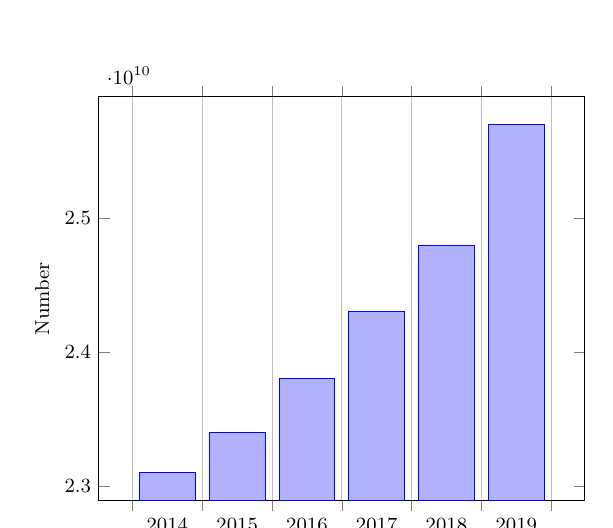
\begin{tikzpicture}[scale=0.9]
            \tikzstyle{every node}=[font=\small,scale=0.9]
            \begin{axis}[
                    x tick label style={/pgf/number format/1000 sep={}},
                    ylabel=Number,
                    enlargelimits=0.08,
                    xticklabels={2014,2015,2016,2017,2018,2019,2020},
                    legend style={at={(0.5,-0.2)},
                            anchor=north,legend columns=6},
                    ybar interval=0.8,
                ]
                \addplot
                coordinates {(2014,23100000000) (2015,23400000000)
                        (2016,23800000000) (2017,24300000000) (2018,24800000000) (2019,25700000000)(2020,25300000000)};
                % \legend{Market size}
            \end{axis}
        \end{tikzpicture}}
    \hspace{10mm}
    \subfigure[Age distribution of programming ]{
    \begin {tikzpicture}[scale = 0.9]
    \tikzstyle{every node}=[font=\small,scale=0.8,align=center]
    \pie [polar]{25/ below \\ 24 , 34/ between \\24-30 , 17/ between \\31-35, 9/ between \\36-40, 15/ over \\ 41}
    \end{tikzpicture}
    }
\end{figure}

\newpage
\section{Growth Trends ln This Business}
\vspace{-0.1cm}
\hrule
\vspace{0.2cm}
Around the World parents as well as educational facilities realize the rising reach of programming and its current relevance in society. Due to the increasing demand for contemporary technologies, youngsters who learn programming, are well qualified to examine circumstances and problems both technically and conceptually.

Initially, the organization operates as a studio, designing lightweight physical hardware and developing logical hardware as a later step. The company's scope will progressively extend from e-commerce platforms to self-built websites in the mid-term. Buyers go to the built-in websites to learn software based on the product's resource material. The company focuses on the development of hardware modules and the matching of software programs. The company will change from a product seller to a programming education and training institution, establishing a series of supporting courses and educating children to accomplish challenging and intriguing projects, if the company can generate regular earnings and has sufficient cash. We will assist children in participating in various competitions within their capacity to exercise themselves in order to increase their project skill in the second half of the semester.

\section{The Vision And The People}
\vspace{-0.1cm}
\hrule
\vspace{0.2cm}
\begin{itemize}
    \setlength{\itemsep}{0pt}
          \setlength{\parsep}{0pt}
          \setlength{\parskip}{0pt}
    \item {\normalsize  Able to manipulate and interpret information from a range of sources, to spot patterns and trends in information and to deduce cause and effect from this.}
    \item  {\normalsize Knows what we do and how we do it. Is aware of our competitors. Up-to-date with general business news. }
    \item  {\normalsize Able to pick up and assimilate relevant information quickly and easily. Learns new tasks rapidly. Responds swiftly and appropriately.}
    \item  {\normalsize Shares information and supports other team members. Can get things done through others and set realistic objectives. Seeks opportunities to develop others.}
    \item {\normalsize Takes balanced view of situations incorporating different perspectives. Reaches logical conclusions and decides on appropriate plan of action.}
    \item {\normalsize Has the ability to recognise information needs and identify and utilise appropriate information sources.}
    \item {\normalsize Able to influence the views and behaviour of others through persuasion and encouragement.}
\end{itemize}

\subsection{Work Experience Related to Business}
\vspace{-0.1cm}
\hrule
\vspace{0.2cm}
\begin{itemize}
    \setlength{\itemsep}{0pt}
          \setlength{\parsep}{0pt}
          \setlength{\parskip}{0pt}
    \item {\normalsize  Mastered basic Software development languages Like JAVA, C++ and hardware development languages like C.}
    \item  {\normalsize Developed executable applications that can be used with small user volumes}
    \item  {\normalsize Used open source hardware for digital circuit building, assembled intelligent control car, spider model, etc.}
    \item  {\normalsize Participated in a research training program and Understood the complete process of building a project.}
\end{itemize}
\subsection{Personal Background and Education Credentials}
\vspace{-0.1cm}
\hrule
\vspace{0.2cm}
\begin{itemize}
    \setlength{\itemsep}{0pt}
          \setlength{\parsep}{0pt}
          \setlength{\parskip}{0pt}
    \item {\normalsize Majored in computer science and technology during college years.}
\end{itemize}

\newpage
\section{Communication}
\vspace{-0.1cm}
\hrule
\vspace{0.2cm}
Due to the Internet nature of startups, the communication equipments are showed as followed:
\begin{itemize}
    \setlength{\itemsep}{0pt}
          \setlength{\parsep}{0pt}
          \setlength{\parskip}{0pt}
    \item {Rent cloud servers to store user data}
    \item {Purchase of basic components for development}
    \item {Commercial rights for software development applications}
    \item {Basic hardware soldering tools and circuit testing tools}
\end{itemize}

\section{Financing}
\vspace{-0.1cm}
\hrule
\vspace{0.2cm}
The overall size of the company's start-up capital is \$100,000, divided into three parts: \textbf{personal contribution(my accountant), partner contribution(partners' accountant), and a bank credit facility(National Bank)}. The specific asset share is shown in Figure 1. For the operation of the capital flow, at the beginning of the company's start-up, it was necessary to purchase the necessary woodworking samples, miniature workbenches, etc. In order to maintain good bank credit and get the bank loan on time, we try to accept some small part-time jobs in software design and construction to maintain the expenses and, to a certain extent, accumulate experience in software design to lay the foundation for independent design and development of websites and software afterwards.

\begin{figure}[h]
    \centering
    \subfigure[Start-up Capital of Company]{
    \begin {tikzpicture}[scale = 0.8]
    \tikzstyle{every node}=[font=\small,scale=0.8,align=center]
    \pie [polar]{35/ Bank\\ Loans , 30/ Partner\\ Assets , 35/ Personal\\  Assets}
    \end{tikzpicture}}
    \hspace{8mm}
    \subfigure[Cash Flow Projection]{
    \begin {tikzpicture}[scale = 0.8]
    \tikzstyle{every node}=[font=\small,scale=0.8,align=center]
    \pie [polar]{30/ recording \\ equipment , 30/ Instructional \\ equipment,20/ Teaching materials \\ purchase, 12/ Video \\ Maintenance ,8/ Ad \\Placement}
    \end{tikzpicture}}
\end{figure}

\section{Acquisitions}
\vspace{-0.1cm}
\hrule
\vspace{0.2cm}
Based on the R\&D-focused nature of the projects undertaken by the Company, i.e. open source, secondary development based on the original content does not give rise to intellectual property rights. The company has a large capital flow, so we need to hire professional accounting staff to take care of the business.

The products include traditional shopping websites (Taobao, etc.) and WeChat mini-programs (customized services). Users can combine their financial conditions and needs to make a purchase. Therefore, there is no need to verify the user's identity.

After being able to maintain normal cash flow, the company will work with small outsourced software companies who will develop and maintain the software, online shopping program, and website; the company will set up a corresponding research and development department, which will be responsible for the design of new hardware building block frames and the assembly of the corresponding mechanical control components.

\section{Marketing}
\vspace{-0.1cm}
\hrule
\vspace{0.2cm}
\subsection{Marketing Plan}
\vspace{-0.1cm}
\hrule
\vspace{-0.2cm}

\begin{figure}[ht]
    \centering  %图片全局居中
    \includegraphics[scale = 0.5]{test.pdf}
    \caption{Children's education programming classification}
\end{figure}

In the early stages of the business, we used a trial lecture by inviting friends and relatives. During the course of lecturing, the curriculum was constantly polished to make it more suitable for children to learn. After the course system is polished and mature, an invitation system is used, and students who are introduced into the course by the students can reduce a small amount of consumption.

In the course, students can either use the existing open source hardware to guide students to carry out simple secondary development, for example, running lights, distance detectors, etc.; or they can combine the developed modules for assembly tests and use the modules to build molded objects, which greatly enhances children's interest in learning. At the same time, we will give children with remarkable learning results the opportunity to be guided by competitions, leading them to make their first appearance in the competition and feel the fun of competition.
\subsection{Advertising and Promotion Plans}
\vspace{-0.1cm}
\hrule
\vspace{0.2cm}

Since enrollment is based on word-of-mouth, it is vital to print paper flyers and recruit volunteers to distribute them on a regular basis in order to broaden the pool of potential consumers and attract additional students interested in mechanical programming. Simultaneously, courses are regularly sold at a discount for a limited time on the company's public phone number and website.

Advertisements are placed to attract potential customers; free experience courses are made up to pique consumers' interest in the courses; and a full set of courses and corresponding communication groups are set up for the delivery of course materials and query counseling.
\subsection{Purchasing and Inventory Control}
\vspace{-0.1cm}
\hrule
\vspace{0.2cm}
Purchase items include: basic hardware development boards, succession logic hardware modules, wires, soldering tools, assembly tools, molded products (for display), office equipment (tables and chairs, etc.), storage boxes, etc. The warehouse mainly stores spare open source hardware devices and related products that have been tested and run.
\section{Growth Program}
\vspace{-0.1cm}
\hrule
\vspace{0.2cm}
\subsection{Expansion}
\vspace{-0.1cm}
\hrule
\vspace{0.2cm}
\begin{enumerate}
    \setlength{\itemsep}{0pt}
          \setlength{\parsep}{0pt}
          \setlength{\parskip}{0pt}
    \item Start-up period \\
          Individuals holding accounting roles and responsible for cash flow probes, with a headcount size of the number of start-up people, provide the resources, as do partner contributions and bank loans.
    \item Developmental period \\
          Increase research activities and be in charge of improving course content as well as secondary hardware development. Attract more funding partners; hire expert accountants for account management; and increase the company's employment to ten workers.
    \item Stabilization period\\
          Students can gradually migrate from single software learning to diversified hardware and software multi-party learning based on domestic hardware for basic secondary development. Improve the curriculum system to develop topic course software, software, and hardware interaction. Create stage competitions and prize pools to motivate students to engage in self-study and share their work.
    \item Cooperation period\\
          Outsource the promotion business and hire a third party to create and maintain the online community as well as design the software platform. In addition to providing offline sessions, hire a fixed number of instructors to film course videos and set up online courses.
\end{enumerate}

\subsection{Handling Major Problems}
\vspace{-0.1cm}
\hrule
\vspace{0.2cm}

Slow down the opening of the research and development department, increase funds for the teaching part, open a variety of course modes, expand the teaching target from the lower grades to the upper grades, offline courses are recorded in real time and converted into online courses to facilitate student consolidation, which can ensure the quality of leaning.

When a single client accounts for more than half of the revenue, we must choose between product and user experience. Diversifying a client base is critical to a company's growth, but it can be tough, especially when the client pays on time and in full. Having a client that is willing to pay for a product or service on time is a blessing for many small businesses.

This agreement helps the customer to avoid the risks associated with adding payroll in an area where activity could dry up at any time. When a single client stops paying, it is often better for a business to have a diverse client base to pick up the slack.
\begin{figure}[ht]
    \centering  %图片全局居中
    \subfigure[Offline Problems]{\includegraphics[scale = 0.22]{show2.pdf}}
    \subfigure[Online Problems]{\includegraphics[scale = 0.22]{show3.pdf}}
    \caption{Major Problem and Solutions}
\end{figure}

\end{document}